\documentclass{article}

\usepackage{graphicx}
\usepackage{tikz}
\usepackage{tikzsymbols}
\usetikzlibrary{calc,patterns,shapes.geometric}
\pagestyle{empty}
\usepackage[margin=0pt]{geometry}
\geometry{papersize={14in,12in}}

\def\centerarc[#1](#2)(#3:#4:#5){\draw[#1] ($(#2)+({#5*cos(#3)},{#5*sin(#3)})$) arc (#3:#4:#5);}

\begin{document}
	\begin{figure}
		\centering
		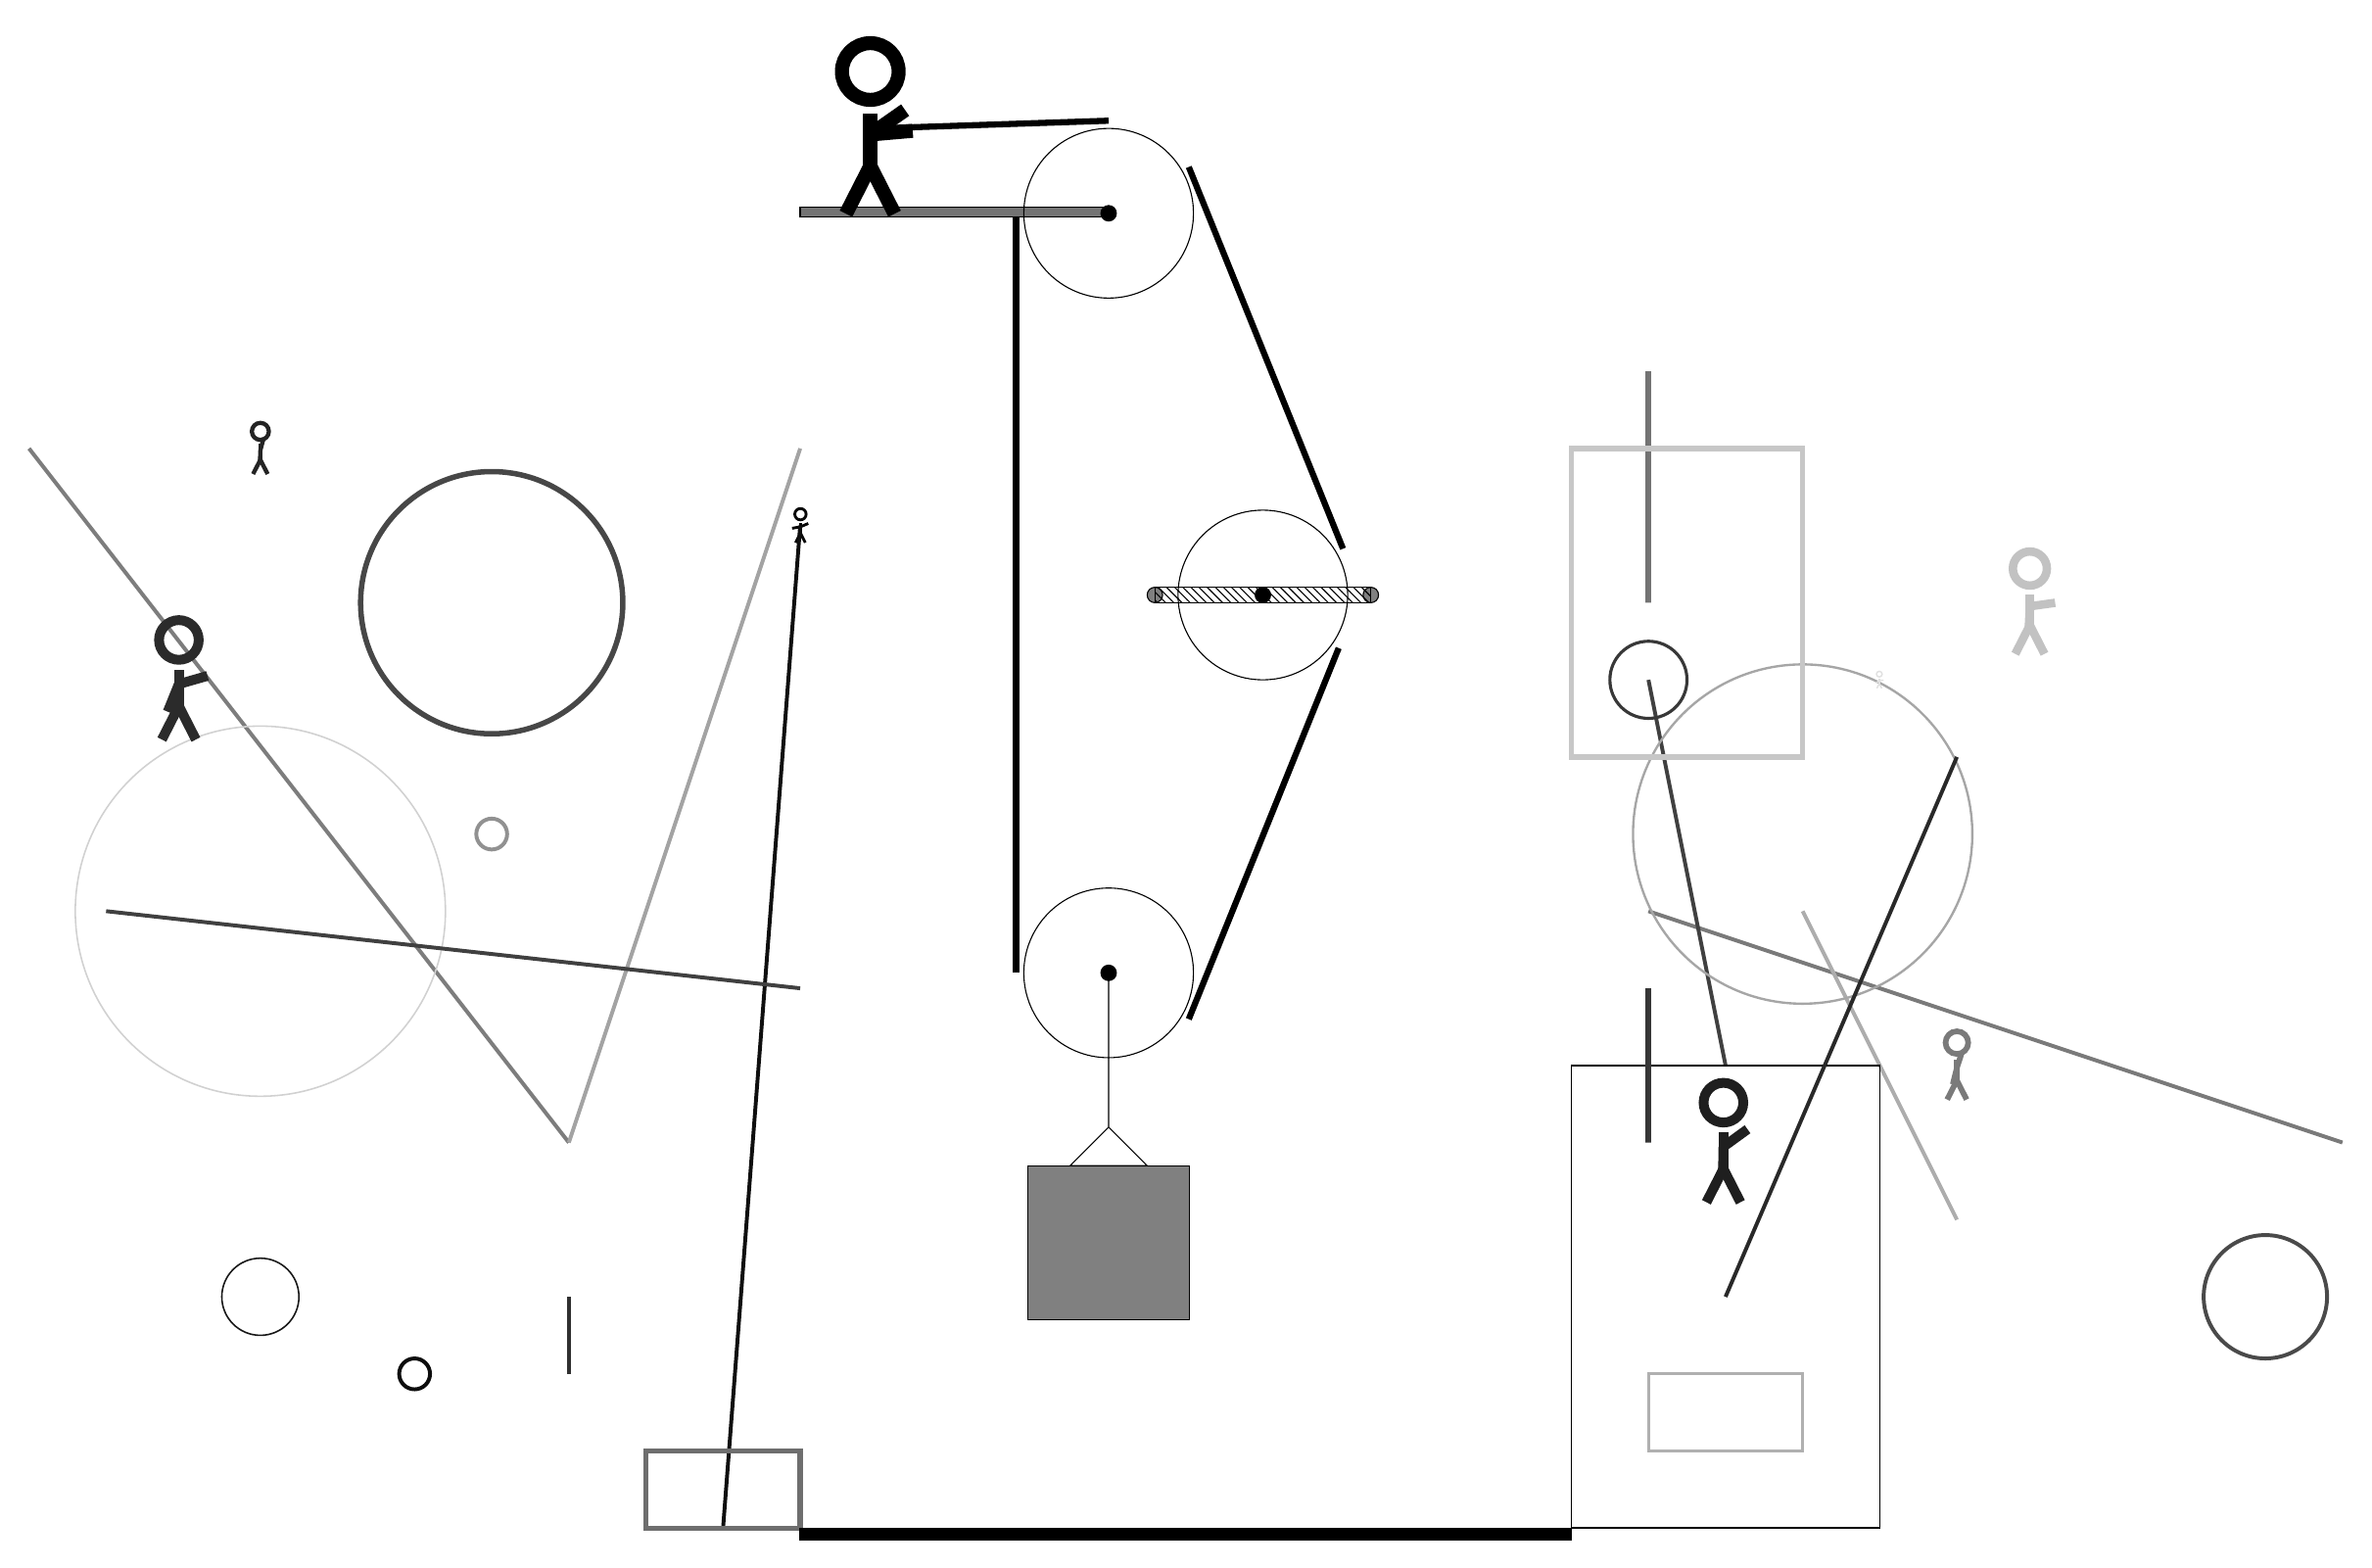
\begin{tikzpicture}
			%%%%% START %%%%%
			
			\draw[fill=black!55] (-2, 14) rectangle (2, 14.125);
			
			\draw (2, 4.2) circle (1.1);
			\draw[fill=black] (2, 4.2) circle (0.1);
			
			\draw[line width=0.5mm, color=black!52](9, 5) -- (18, 2);
			
			\node[line width=0.6mm, color=black!52] at (13, 3) {\Strichmaxerl[4][76][72]};
			\node[line width=0.7mm, color=black!97] at (-2, 10) {\Strichmaxerl[2][10][23]};
			\draw[line width=0.5mm, color=black!75](10, 3) -- (9, 8);
			\draw[line width=0.5mm, color=black!51](-5, 2) -- (-12, 11);
			
			\draw [line width=0.5mm, color=black!71](17, 0) circle (0.8);
			\draw[line width=0.5mm, color=black!32](13, 1) -- (11, 5);
			
			\draw[line width=0.5mm, color=black!94](-2, 10) -- (-3, -3);
			\node[line width=0.4mm, color=black!88] at (10, 2) {\Strichmaxerl[7][89][36]};
			\draw [line width=0.3mm, color=black!35](11, 6) circle (2.2);
			\draw [line width=0.5mm, color=black!95](-7, -1) circle (0.2);
			\draw[line width=0.2mm, color=black!100] (8, -3) rectangle (12, 3);
			\draw [line width=0.2mm, color=black!91](-9, 0) circle (0.5);
			
			\draw[line width=0.4mm, color=black!31] (9, -1) rectangle (11, -2);
			\draw[line width=0.5mm, color=black!81](-5, -1) -- (-5, 0);
			\node[line width=0.5mm, color=black!24] at (14, 9) {\Strichmaxerl[6][87][8]};
			\draw [line width=0.2mm, color=black!18](-9, 5) circle (2.4);
			\draw[line width=0.7mm, color=black!57] (-2, -2) rectangle (-4, -3);
			\draw[line width=0.7mm, color=black!55] (9, 9) rectangle (9, 12);
			\draw[line width=0.7mm, color=black!79] (9, 2) rectangle (9, 4);
			\draw[line width=0.5mm, color=black!84](10, 0) -- (13, 7);
			
			\draw [line width=0.4mm, color=black!78](9, 8) circle (0.5);
			\draw [line width=0.5mm, color=black!43](-6, 6) circle (0.2);
			\node[line width=0.6mm, color=black!12] at (12, 8) {\Strichmaxerl[1][39][3]};
			\draw[line width=0.5mm, color=black!36](-5, 2) -- (-2, 11);
			
			\draw [line width=0.7mm, color=black!72](-6, 9) circle (1.7);
			\draw[line width=0.5mm, color=black!75](-2, 4) -- (-11, 5);
			\draw[line width=0.7mm, color=black!22] (8, 11) rectangle (11, 7);
			\node[line width=0.3mm, color=black!86] at (-9, 11) {\Strichmaxerl[3][88][75]};
			\node[line width=0.4mm, color=black!83] at (-10, 8) {\Strichmaxerl[7][68][16]};
			
			\draw (2, 14.05) circle (1.1);
			\draw[fill=black] (2, 14.05) circle (0.1);
			
			\draw[fill=white](4, 9.1) circle (1.1);
			\draw[fill=black] (4, 9.1) circle (0.1);
			\draw[fill=black!50] (2.6, 9.1) circle (0.1);
			\draw[fill=black!50] (5.4, 9.1) circle (0.1);
			\draw[pattern=north west lines, pattern color=black] (2.6, 9.2) rectangle (5.4, 9.0);
			
			\draw (2, 4.2) -- (2, 2.2) -- (1.5, 1.7) -- (2.5, 1.7) -- (2, 2.2);
			\draw[fill=black!50] (0.95, 1.7) rectangle (3.05, -0.3);
			
			\draw[line width=0.8mm] (0.8, 14) -- (0.8, 4.2);
			\centerarc[line width=0.8mm](2, 4.2)(180:330:1.2000000000000002);
			\draw[line width=0.8mm](3.0392, 3.6) -- (4.983, 8.4117);
			\centerarc[line width=0.8mm](4, 9.1)(390:325:1.2000000000000002);
			\draw[line width=0.8mm](5.0392, 9.7) -- (3.0392, 14.65);
			\centerarc[line width=0.8mm](2, 14.05)(30:90:1.2000000000000002);
			\draw[line width=0.8mm](2, 15.25) -- (-1, 15.15);
			
			\node at (-1, 15.15) {\Strichmaxerl[10][-175][35]};
			
			\draw[fill=black] (-2, -3) rectangle (8, -3.15);
			
			%%%%% END %%%%%
		\end{tikzpicture}
	\end{figure}	
\end{document}